\documentclass[tikz]{standalone}

\usepackage{fontspec}

\usetikzlibrary{arrows}
\usetikzlibrary{calc}
\usetikzlibrary{decorations.pathreplacing}
\usetikzlibrary{positioning}
\usetikzlibrary{matrix}

\usepackage{fontspec}

\begin{document}

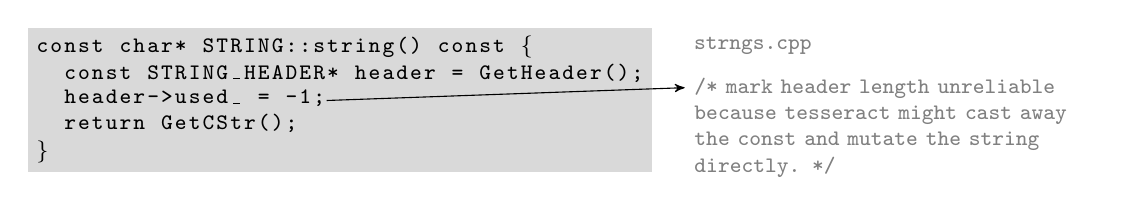
\begin{tikzpicture}
  [node distance=5mm, >=stealth',
  every node/.style={font=\footnotesize},
  every matrix/.style={fill=black!15, inner sep=1mm, row sep=0.5mm,
                        matrix of nodes, nodes in empty cells,
                        minimum height=0.5em, minimum width=.5em,
                        nodes={anchor=base, inner sep=0, font=\ttfamily\footnotesize}}]

  \matrix (snippet) {
c & o & n & s & t &   & c & h & a & r & * &   & S & T & R & I & N & G & : & : & s & t & r & i & n & g & ( & ) &   & c & o & n & s & t &   & \{ &   &   &   &   &   &   &   &   \\
  &   & c & o & n & s & t &   & S & T & R & I & N & G & \_ & H & E & A & D & E & R & * &   & h & e & a & d & e & r &   & = &   & G & e & t & H & e & a & d & e & r & ( & ) & ; \\
  &   & h & e & a & d & e & r & - & > & u & s & e & d & \_ &   & = &   & - & 1 & ; &   &   &   &   &   &   &   &   &   &   &   &   &   &   &   &   &   &   &   &   &   &   &   \\
  &   & r & e & t & u & r & n &   & G & e & t & C & S & t & r & ( & ) & ; &   &   &   &   &   &   &   &   &   &   &   &   &   &   &   &   &   &   &   &   &   &   &   &   &   \\
\} &   &   &   &   &   &   &   &   &   &   &   &   &   &   &   &   &   &   &   &   &   &   &   &   &   &   &   &   &   &   &   &   &   &   &   &   &   &   &   &   &   &   &   \\
  };

  \node (comment) [right=of snippet-3-44.base, black!50, xshift=1mm, yshift=-3mm, align=left, text width=5cm] {\ttfamily /* mark header length unreliable because tesseract might cast away the const and mutate the string directly. */};

 \node [above, anchor=west, black!50, xshift=0.5cm]
        at (snippet-1-44.north east)
        {\texttt{strngs.cpp}};
  \draw [->] let \p1 = (snippet-3-21.east),
                 \p2 = ($ (comment.north west) + (0, -2.5mm) $)
              in (\p1) -- (\p2);

\end{tikzpicture}

\end{document}
